\documentclass[a4paper,10pt]{article}
\usepackage[utf8x]{inputenc}
\usepackage{graphicx}

%opening
\title{Trainmining}
\author{}

\begin{document}

\maketitle

\begin{abstract}

\end{abstract}

\section{Introduction}\label{sec:context}
Maintenance is one of the most important tasks to assure the quality and correct operation of any kind of system. Even the highest quality systems, built by the best engineers to operate for long periods with the least possible human assistance, will eventually be exposed to damage or malfunction. In order to avoid the negative effects that system malfunction can produce, a significant amount of resources and effort is usually needed to be put on maintenance tasks. However, putting resources and effort on maintenance procedures might still not be enough if the procedures and strategies are not adequate and efficient.

Traditionally, we have discerned between two types of maintenance procedures:

\emph{Corrective maintenance} is the most common approach, although it has very important limitations. With this approach, elements of our system are repaired or replaced once they have failed or worn out, to bring them back to operation. This usually means a high downtime in operation, as no actions are taken until our system is already malfunctioning.

\emph{Preventive maintenance} focuses on preventing these failures. Elements can be periodically examined and analysed in order to control their operation and perform simpler procedures to adjust them before reaching malfunction and downtime. This approach means much higher costs, as a significantly bigger amount of time is needed to monitor the elements on our system and correct them. However, as downtime means business losses in almost all cases, these higher costs usually pay back in terms of loss reduction.

A balance can be easily achieved by spending on preventive maintenance not more than the losses we would suffer from downtime if we were using a corrective approach.

However, the costs of \emph{preventive maintenance} can be drastically reduced by optimising procedures and using the adequate techniques. For example, we can reduce the amount of variables and magnitudes we are monitoring (and which cost us money to monitor) if we know which ones give the better insight on the status on our systems. The same can be done with corrective maintenance. If we can somehow foresee which systems are going to fail, we can be prepared and reduce impact on our business even if we cannot do anything to prevent its failure.

In both cases, \emph{prediction} can be a key element for maintenance optimisation. Either we know which are the indicators of a system deterioration which we can repair, or we know which systems are going to fail and when to be prepared and optimise corrective procedures. We can even speak of a new type of maintenance - \emph{predictive maintenance} - which embraces several techniques to try and obtain this knowledge of future events.

\section{Project overview}
\emph{Trainmining} aims to implement predictive maintenance techniques on already-existing maintenance stations of a railway network. These maintenance stations monitor different elements and subsystems over a railway line and raises alarms whenever a line element fails or requires human intervention. Additionally, maintenance workers perform different preventive maintenance procedures, gathering information about several parameters on each element and performing the appropriate actions when needed. Acquisition of values and determination of necessary actions is however not automatised within the maintenance stations, and workers have to manually perform these tasks.

In order to design \emph{predictive procedures} for the railway network, we have a big amount of event logs gathered by the maintenance stations, as well as registries filled by maintenance workers when performing preventive tasks. We will therefore try to extract, from that large amount of data, knowledge on how to predict future events from current observations

In this directon, \emph{Data Mining} techniques can be extremely useful in order to find relations between patterns in environment variables and the occurrence of events, or even relations between events themselves. These relations, which may at first not be apparent for the human mind, can be obtained through different automated learning processes, and thus infer markers which will act as indicators of when and how failures can happen. In order to extract this data, we will need to count on a significantly high amount of previous data, gathered during previous years, from which we will apply said techniques.

\section{Objectives}
\subsection{Alarm-based prediction}
\subsubsection{Association sequential rules}
\subsubsection{Station type differentiation}
\subsubsection{Prediction confidence definition}

\subsection{Measuring-based prediction}

\section{Database description}
As mentioned in section~\ref{sec:context}, we will count on two different types of databases. First of all, a database gathering a timeline of alarms (failures and other events which require assistance) and a database gathering environment variables which can act as indicators for the alarms. Both types of databases will be present for each maintenance station present in the system.

\subsection{Alarm database}
The alarm database has is structured as follows:
\subsubsection*{Table ER\_ERRORS}
Contains every alarm received by the Maintenance Station. Has the following fields:
\begin{itemize}
 \item DVNI\_ERRORNUMBER - Alarm identifier
 \item DVNS\_ERRORTIME - Timestamp for the alarm
 \item DVNI\_INSTALLATIONCODE - Code of the installation in which the alarm was raised
 \item DVNI\_SENDERINSTALLATIONCODE - Code of the installation from which the alarm was sent (might be different from the one which raised it)
\end{itemize}

\subsubsection*{Table IG\_INSTALLATIONGENERAL}
This table contains information on all the installations. Has the following fields:
\begin{itemize}
 \item DVNI\_INSTALLATIONCODE - Installation identifier
 \item DVNI\_SYSTEMCODE - Type of system, as defined in the ``SG\_SYSTEMSGENERAL'' table
 \item DVNI\_VERSION - System version
 \item DVAC\_SHORTNAME - Short name of the installation
 \item DVAC\_INSTALLATIONNAME - Name of the installation
 \item DVAC\_LOCATION - Location for the installation
 \item CHK\_IS\_NODE - Whether it is a node (doesn't directly send alarms, only raise them) or not
\end{itemize}

\subsubsection*{Table IG\_NODO\_INSTALLATION}
This table gathers additional information on installations which are nodes. This is, installations that can raise alarms but need a Parent installation to send them. Has the following fields:
\begin{itemize}
 \item IG\_NODO\_INSTALLATION - Identifier of the installation which is a node
 \item DVNI\_FATHER\_INSTALLATION - Identifier of the parent installation
\end{itemize}

\subsubsection*{Alarm information tables ERH\_ERRORS\_HSL1 or ERS\_ERRORS\_SAM\_ENCE}
Both these tables record information on the alarms. Either one or other table is filled depending on which version of the system is installed in the station. However, in terms of information, both contain the following fields:
\begin{itemize}
 \item DVNI\_ERRORNUMBER - Alarm identifier
 \item MESSAGE\_ID - Unique alarm identifier
 \item MESSAGE\_TYPE - Type of alarm, always set as ``notification'' (not relevant)
 \item INVOKE\_TYPE - Tells whether the alarm has generated itself due to a connection or disconnection (if type is ``node'') or is generated by a diagnosis system (``saml'') or energy system (``energy'')
 \item INVOKE\_NAME - Irrelevant, always set to ``diagnosis''
 \item EVENT\_TYPE - Defines the type of alarm which has been generated. Its possible values will be described afterwards.
 \item ADDITIONAL\_TEXT - Alarm code
 \item ADDITIONAL\_INFOS - Additional parameters to be shown in error message
 \item DVNI\_ERRORCATEGORY - Alarm severity. Values from 1 to 5 indicating importance of the alarm, or -1 if the alarm indicates recovery from a previous failure.
\end{itemize}
The ``ERH\_ERRORS\_HSL1'' table, has one additional field:
\begin{itemize}
 \item CLAZZ - Shows the type of system which has sent the alarm
\end{itemize}
The field ``EVENT\_TYPE'' can have one of the following values:
\begin{itemize}
  \item fieldElementAlarm - Alarm related to a field element
  \item fieldElementFailure - Failure in a field element
  \item operatorInformation - Information to the operator
  \item imCpuAndCommunications - Related to IM CPU or IM communications
  \item internalDiagnosis - Internal diagnosis of a system
  \item operationsDiagnosisCommunications - Communication error in Operation and Diagnosis systems
  \item ImFecVersions - IM or FEC version
  \item internalTraces - Internal traces of a system
  \item operatorCommandAnswer - Answer to an operator command
  \item CommProblem - Undefined communication problem
  \item Information - Information message: versions, etc.
  \item CommunicationsAlarm - Procedures and processes to carry information from one point to other
  \item QualityOfServiceAlarm - Loss of quality of service
  \item ProcessingErrorAlarm - SW or processing error
  \item EquipmentAlarm - Equipment failure
  \item EnvironmentAlarm - Related to the environment where the system is located
  \item other - Other
\end{itemize}

\subsection{First insight in provided databases}
\subsubsection{Alarm classification}
In order to have a better insight of the provided databases and the mentioned descriptions, a preliminary insight was made, quantitatively analysing some of the parameters which seemed more relevant for alarm definition. Specifically, the chosen parameters are the following:

\begin{itemize}
 \item EVENT\_TYPE
 \item INVOKE\_TYPE
 \item DVNI\_ERRORCATEGORY (Error Category)
\end{itemize}

The proportion of each kind of alarms in each of the provided databases (Antequera, Camas, Segovia and Sevilla) is as follows:
\begin{figure}[ht!]
 \centering
 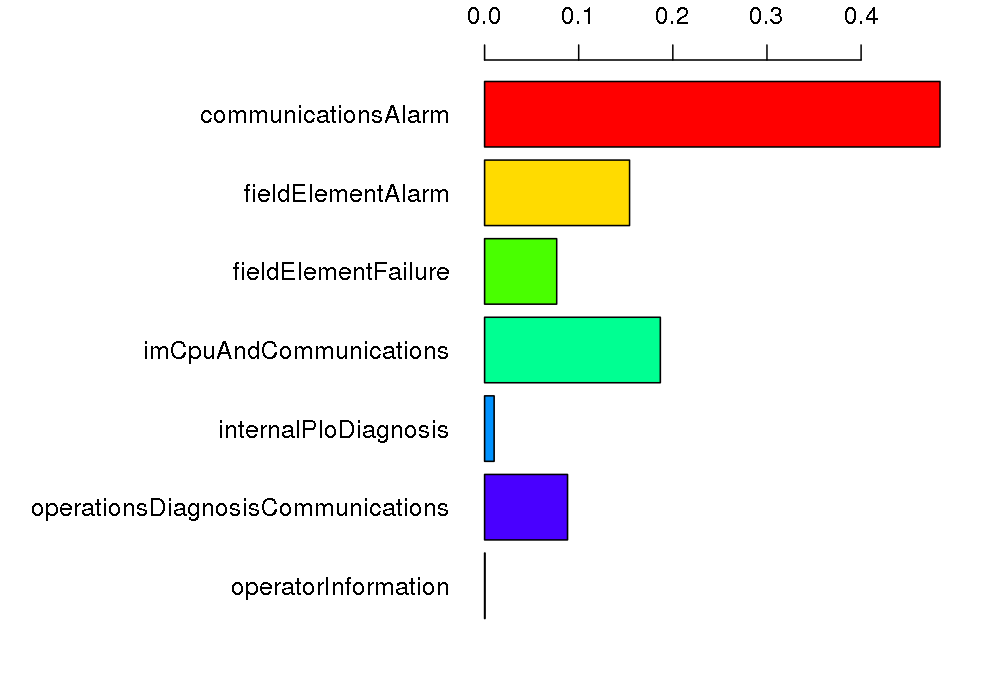
\includegraphics[width=\textwidth]{./img/antequera_graph.png}
 \caption{Alarm information for Antequera}
 \label{fig:anteq}
\end{figure}
\begin{figure}[ht!]
 \centering
 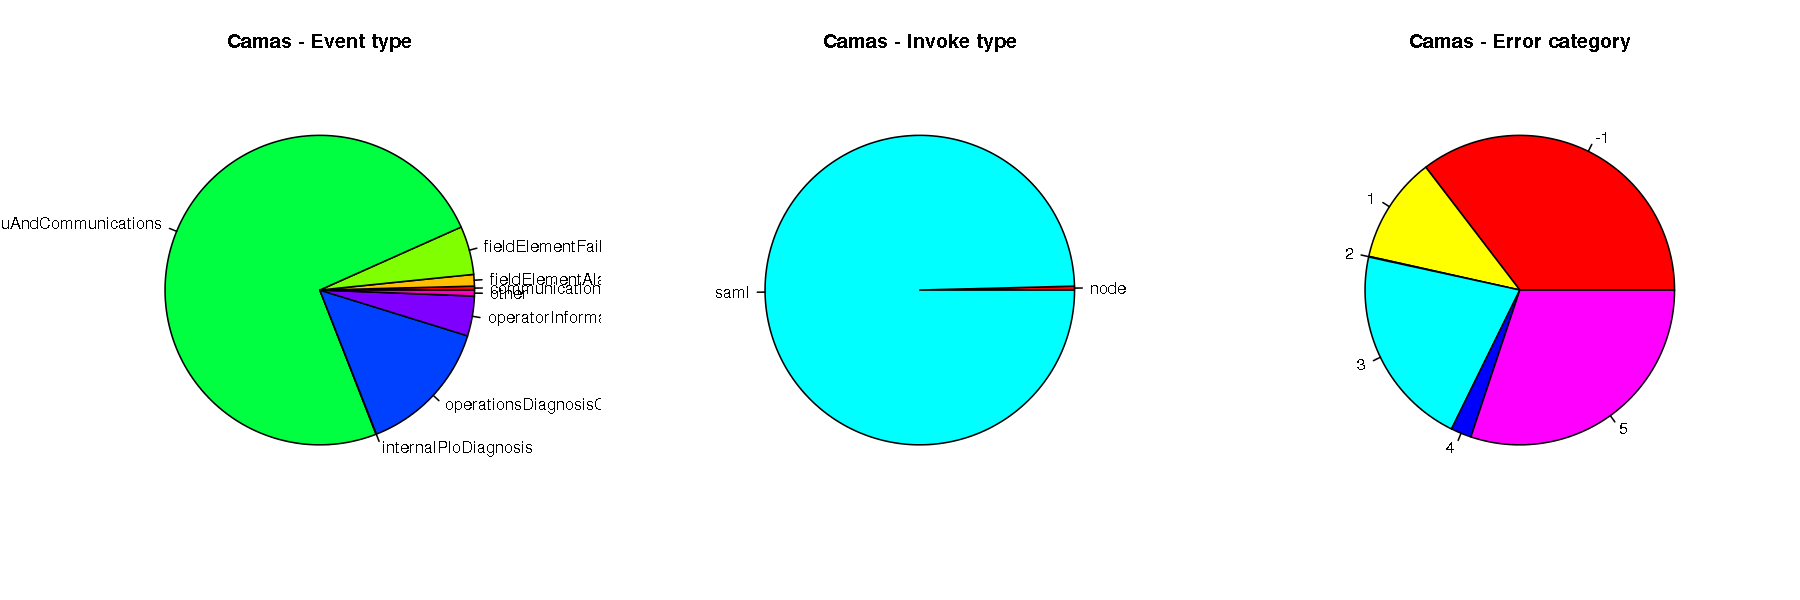
\includegraphics[width=\textwidth]{./img/camas_graph.png}
 \caption{Alarm information for Camas}
 \label{fig:camas}
\end{figure}
\begin{figure}[ht!]
 \centering
 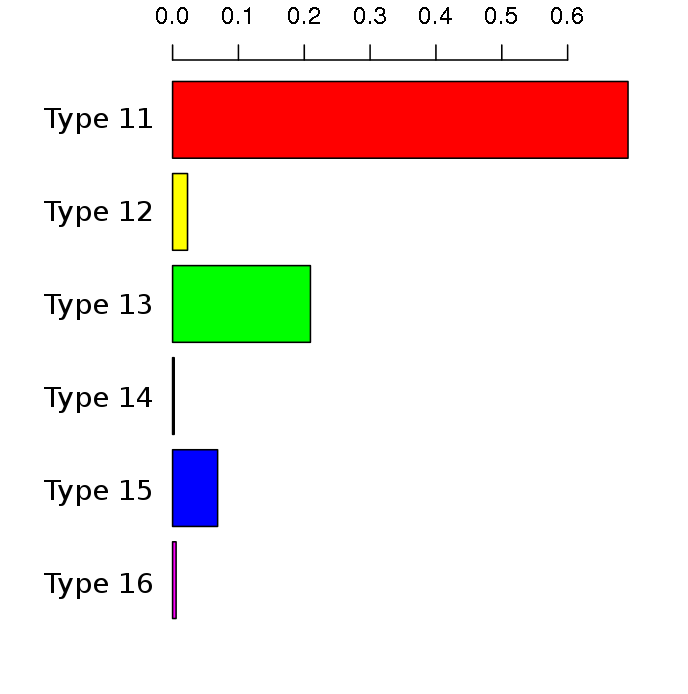
\includegraphics[width=\textwidth]{./img/segovia_graph.png}
 \caption{Alarm information for Segovia}
 \label{fig:segovia}
\end{figure}
\begin{figure}[ht!]
 \centering
 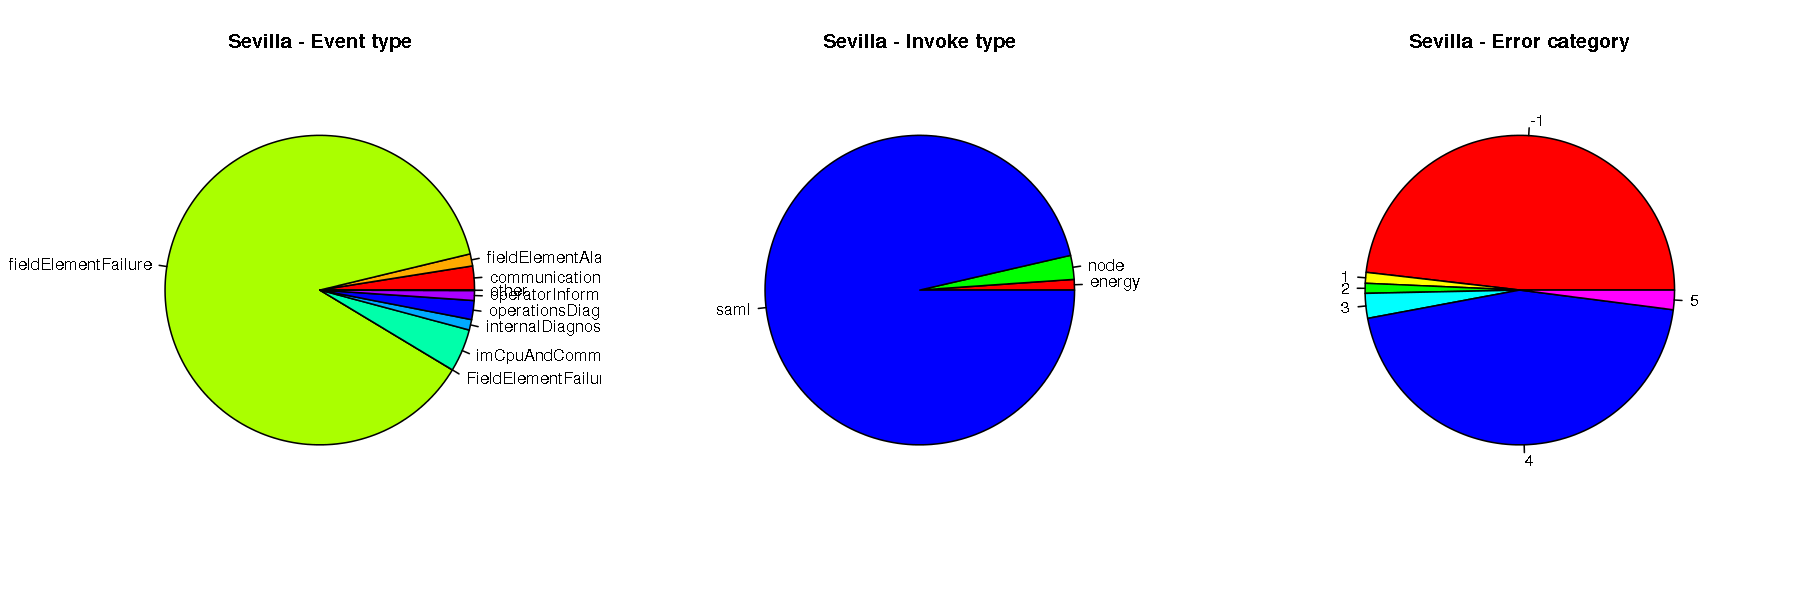
\includegraphics[width=\textwidth]{./img/sevilla_graph.png}
 \caption{Alarm information for Sevilla}
 \label{fig:sevilla}
\end{figure}

\subsubsection{Hourly timeline}

In order to make a first approach to data analysis, we decided to analyse the alarms on a hourly distribution, checking which types of alarms are more likely to happen in different hours during the day. The result is the following:

\clearpage

\begin{figure}[h!]
 \centering
 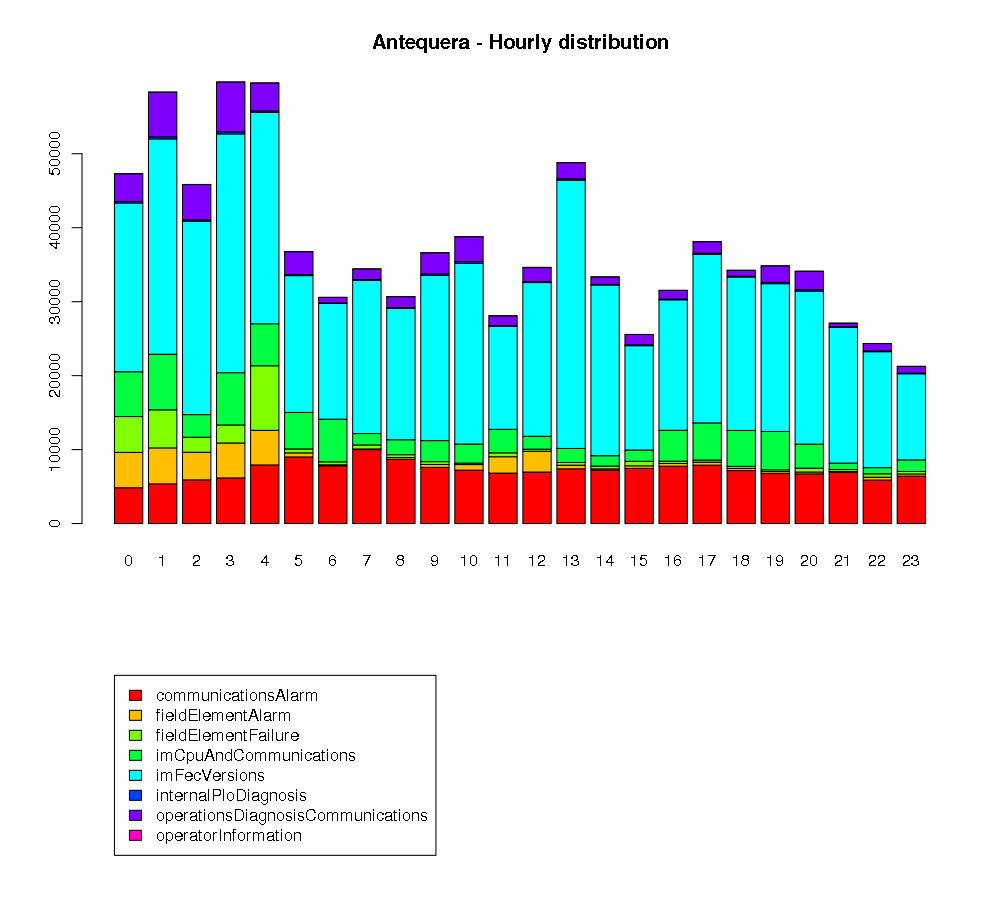
\includegraphics[height=0.4\textheight]{./img/antequera_timeline.png}
 \caption{Hourly distribution for Antequera (stacked)}
\end{figure}
\begin{figure}[h!]
 \centering
 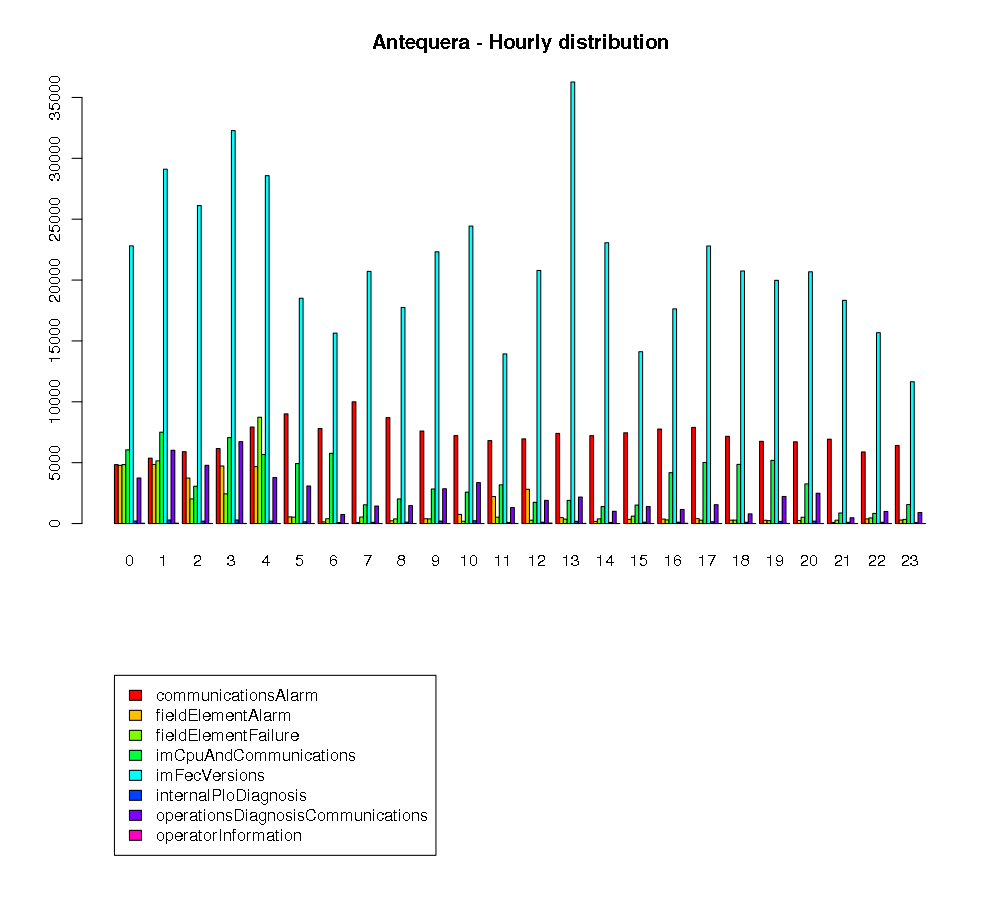
\includegraphics[height=0.4\textheight]{./img/antequera_timeline_b.png}
 \caption{Hourly distribution for Antequera}
\end{figure}

\begin{figure}[h!]
 \centering
 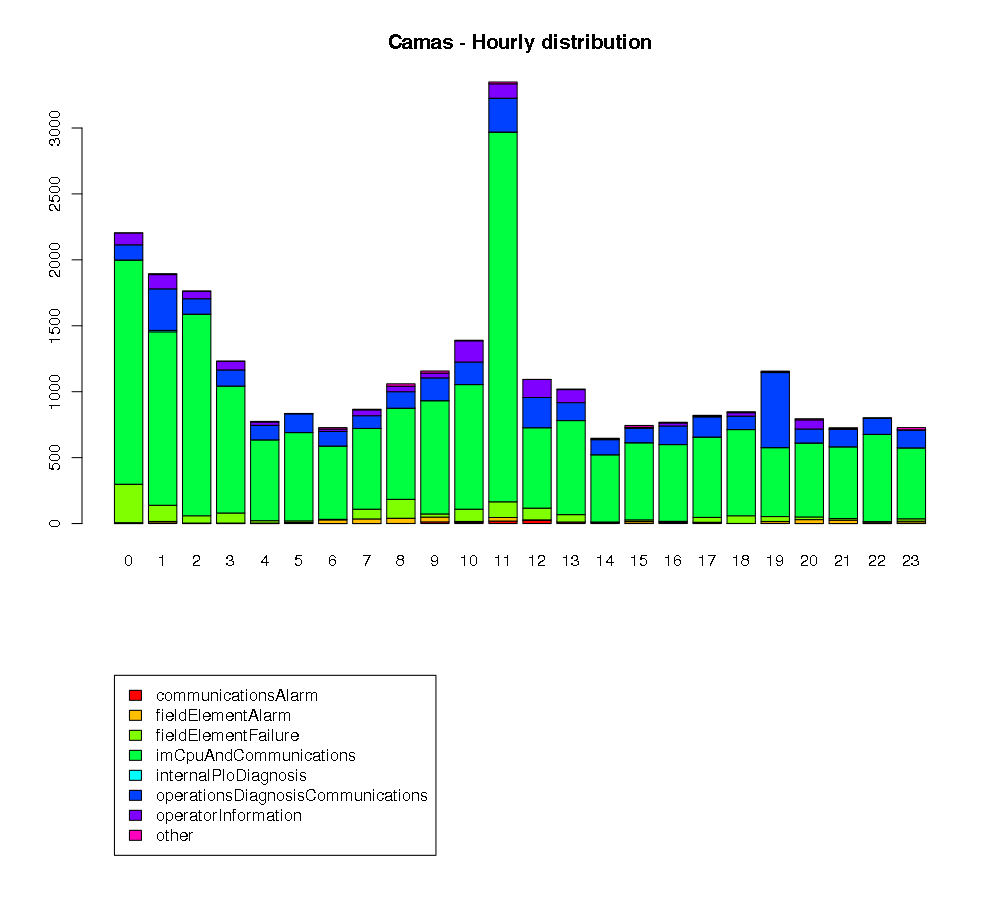
\includegraphics[height=0.4\textheight]{./img/camas_timeline.png}
 \caption{Hourly distribution for Camas (stacked)}
\end{figure}
\begin{figure}[h!]
 \centering
 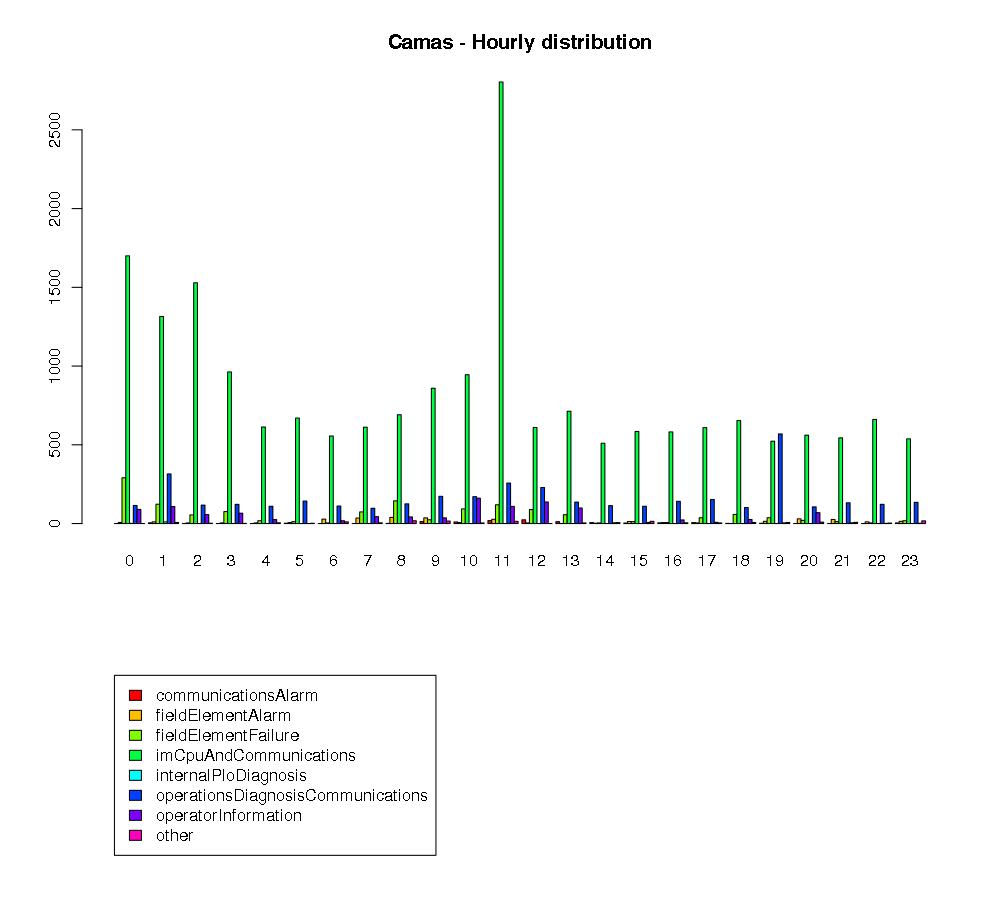
\includegraphics[height=0.4\textheight]{./img/camas_timeline_b.png}
 \caption{Hourly distribution for Camas}
\end{figure}

\begin{figure}[h!]
 \centering
 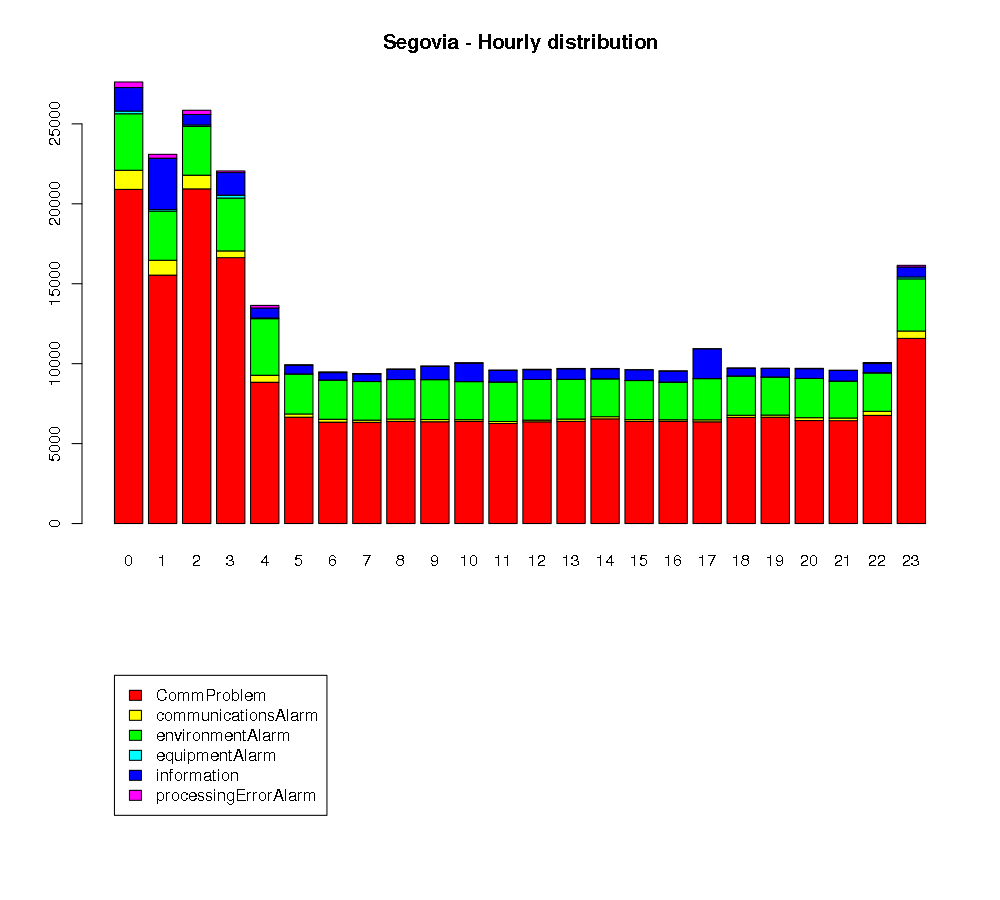
\includegraphics[height=0.4\textheight]{./img/segovia_timeline.png}
 \caption{Hourly distribution for Segovia (stacked)}
\end{figure}
\begin{figure}[h!]
 \centering
 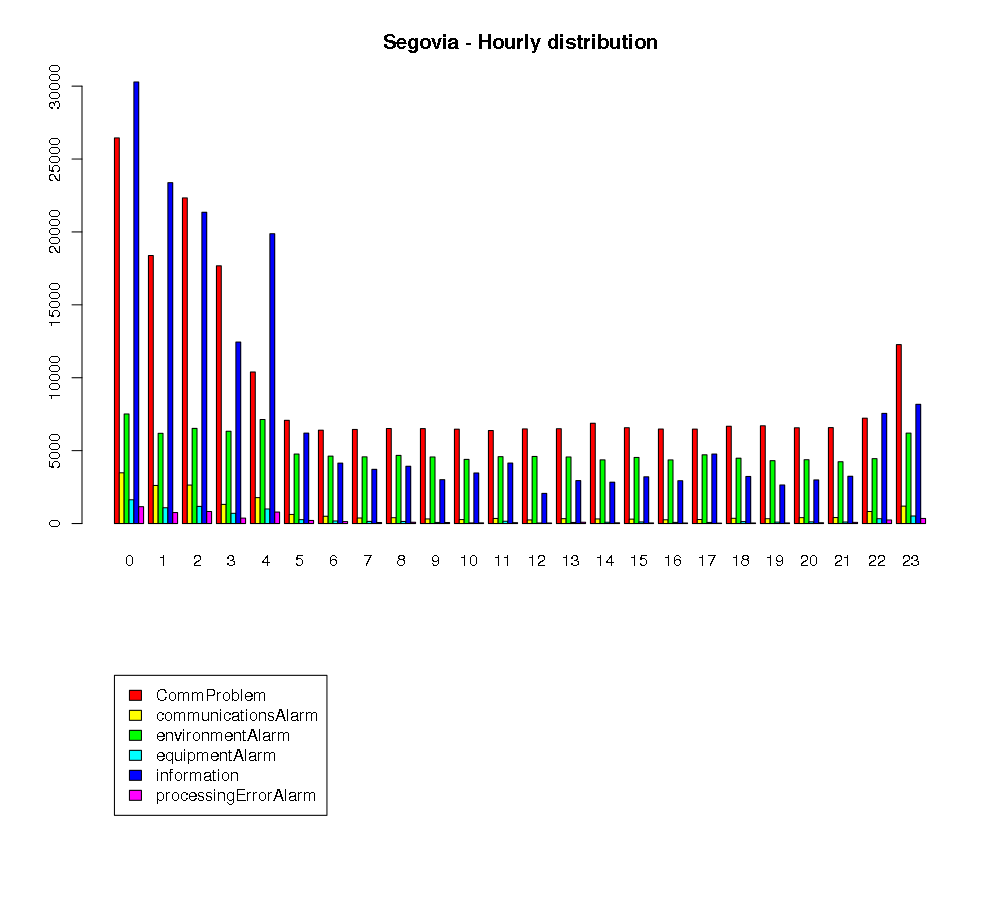
\includegraphics[height=0.4\textheight]{./img/segovia_timeline_b.png}
 \caption{Hourly distribution for Segovia}
\end{figure}

\begin{figure}[h!]
 \centering
 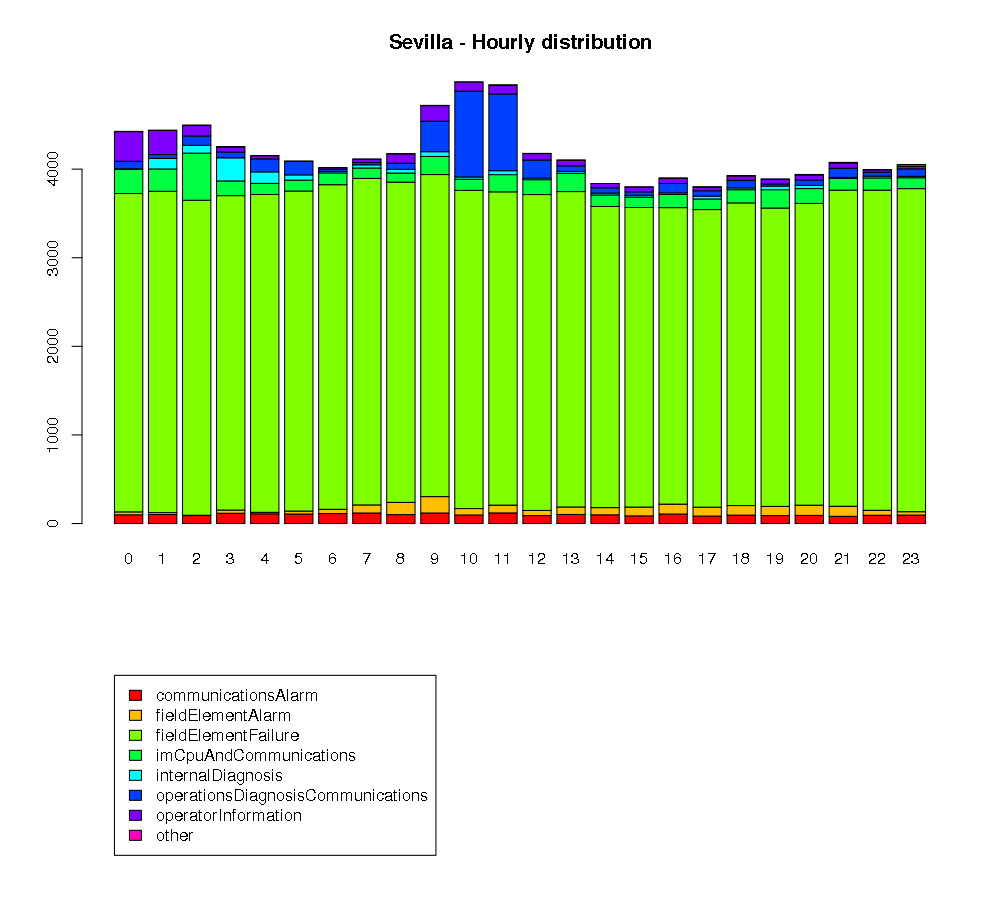
\includegraphics[height=0.4\textheight]{./img/sevilla_timeline.png}
 \caption{Hourly distribution for Sevilla (stacked)}
\end{figure}
\begin{figure}[h!]
 \centering
 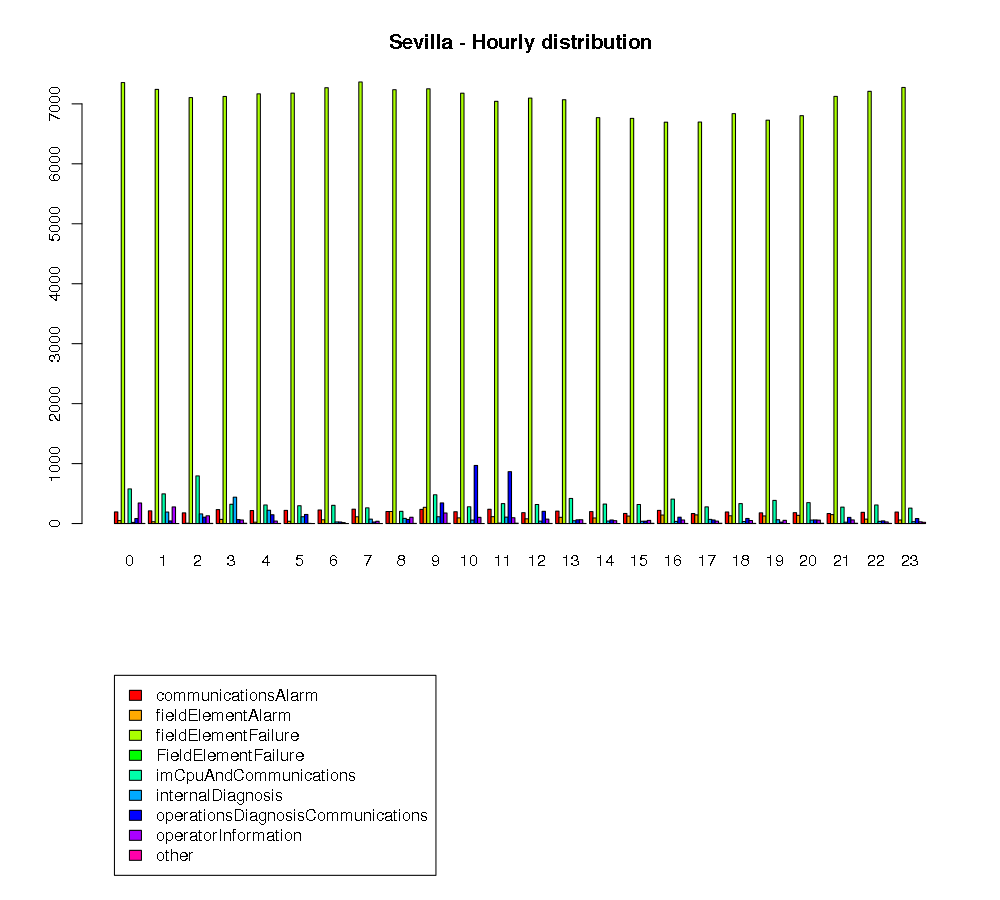
\includegraphics[height=0.4\textheight]{./img/sevilla_timeline_b.png}
 \caption{Hourly distribution for Sevilla}
\end{figure}

\clearpage

\subsubsection{Daily correlation}

We have also generated graphics for correlation between number of alarms of each type during the day, and occurrences of other types of alarms. The result is as follows:

\begin{figure}[h!]
 \centering
 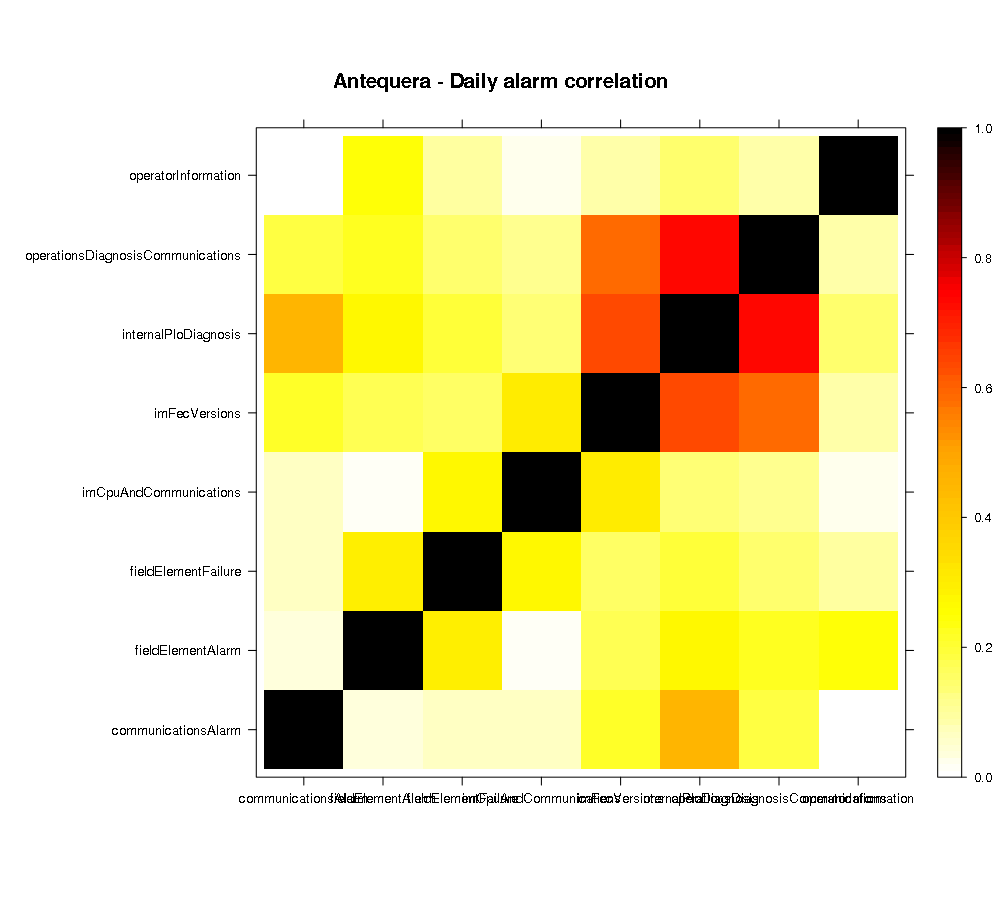
\includegraphics[height=0.4\textheight]{./img/antequera_correlation.png}
 \caption{Daily correlation for Antequera}
 \label{fig:anteq}
\end{figure}
\begin{figure}[h!]
 \centering
 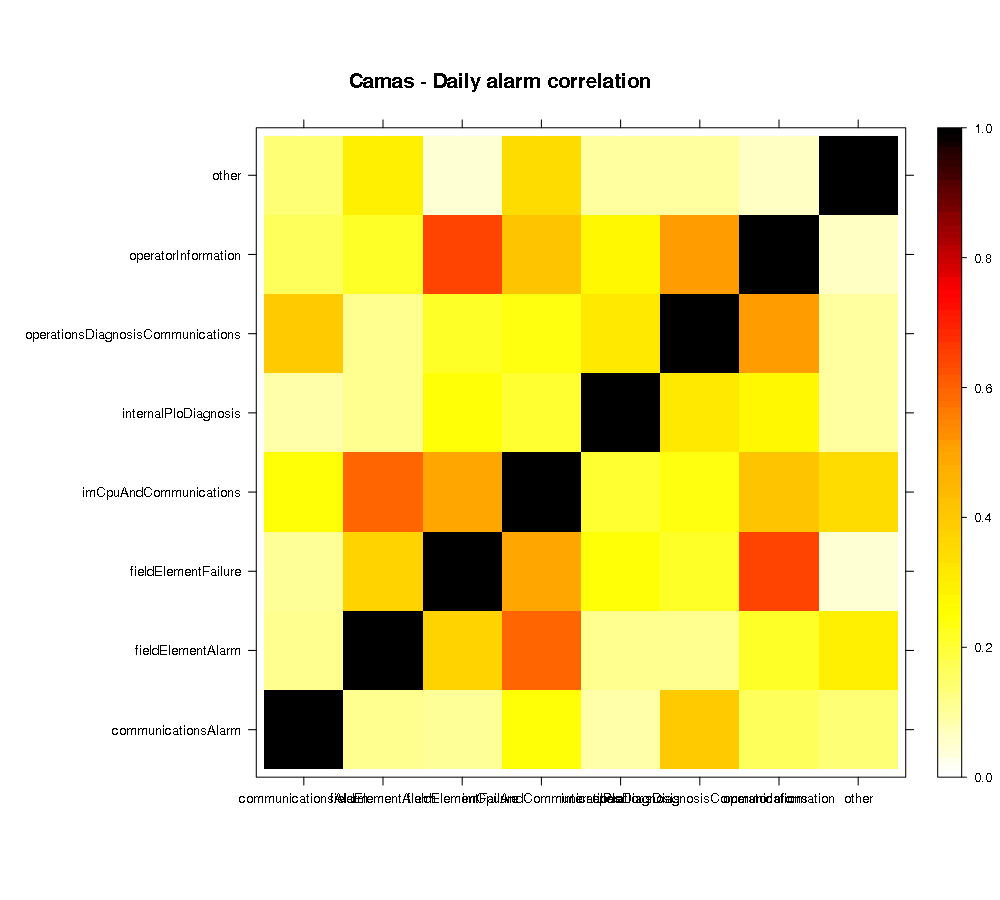
\includegraphics[height=0.4\textheight]{./img/camas_correlation.png}
 \caption{Daily correlation for Camas}
 \label{fig:camas}
\end{figure}
\begin{figure}[h!]
 \centering
 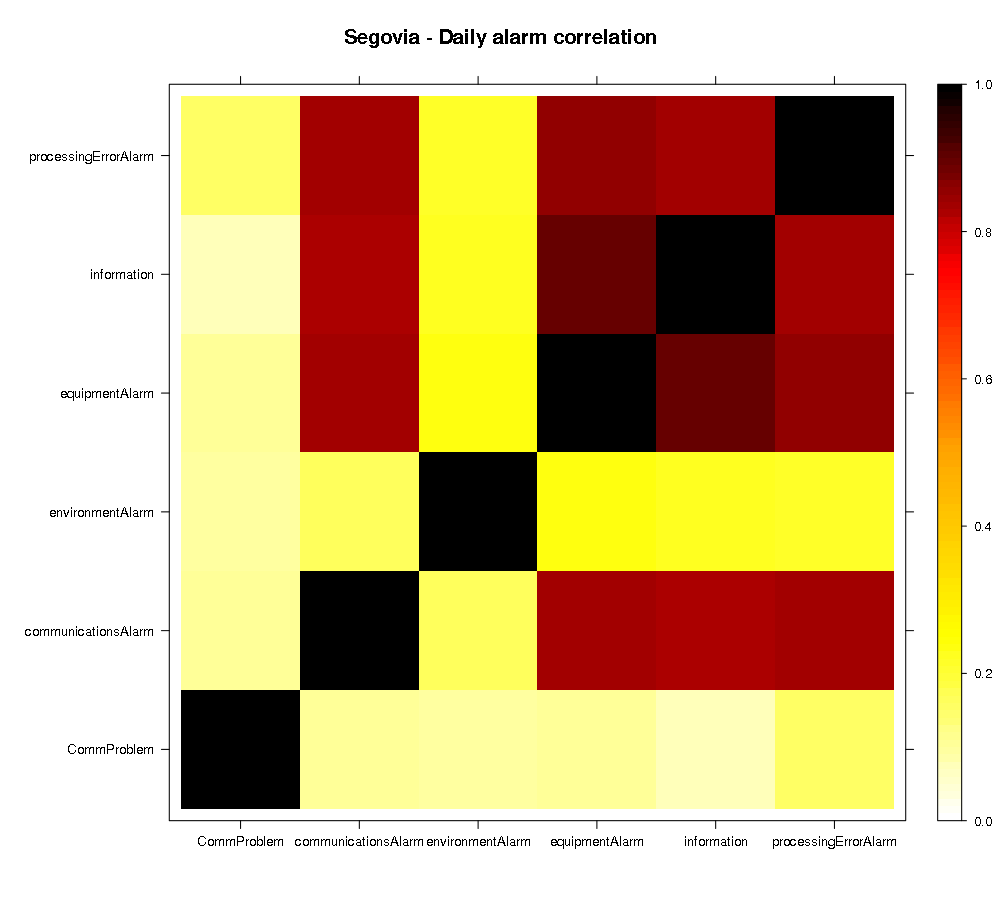
\includegraphics[height=0.4\textheight]{./img/segovia_correlation.png}
 \caption{Daily correlation for Segovia}
 \label{fig:segovia}
\end{figure}
\begin{figure}[h!]
 \centering
 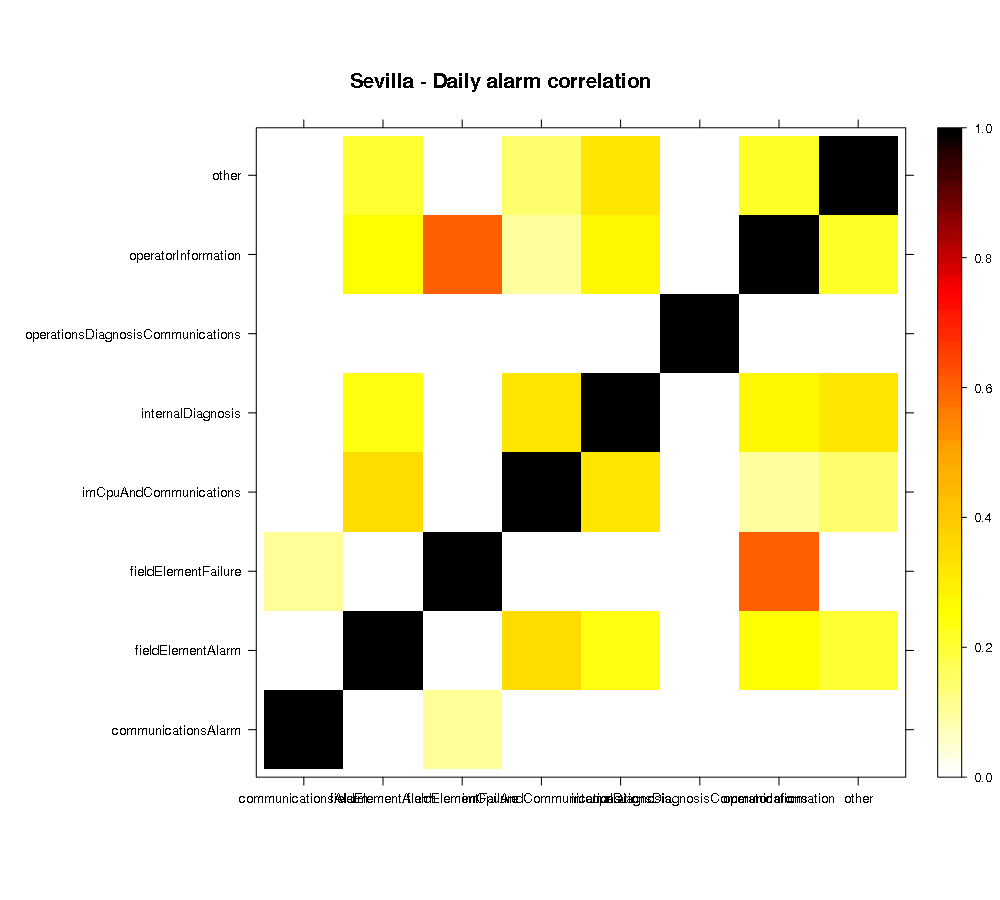
\includegraphics[height=0.4\textheight]{./img/sevilla_correlation.png}
 \caption{Daily correlation for Sevilla}
 \label{fig:sevilla}
\end{figure}

\clearpage

In this first approach, we see that this correlation is not consistent between the different databases. Therefore, information cannot be directly inferred from these results, and additional analysis will be necessary.


\end{document}
